\newpage
\section{Обзор предметной области}
\label{review}

\subsection{Методы фильтрации спама}
\subsubsection{схема работы E-Mail}
Для того, чтобы понять где и как можно бороться со спамом необходимо разобраться с общей схемой работы электронной почты, которая определена в \cite{RFC2081}. Пусть пользователь $A$ отправляет пользователю $B$ письмо. Ниже приведена типичная последовательность действий, которые выполняются между моментами времени, в который $A$ нажимает кнопку ``отправить'' в своем почтовом клиенте и моментом времени, когда $B$ видит письмо в своем почтовом клиенте. Пусть для определенности $A$ имеет адрес foo@bar.net, а $B$ имеет почтовый адрес b@example.com.

\begin{figure}[h]
\begin{center}
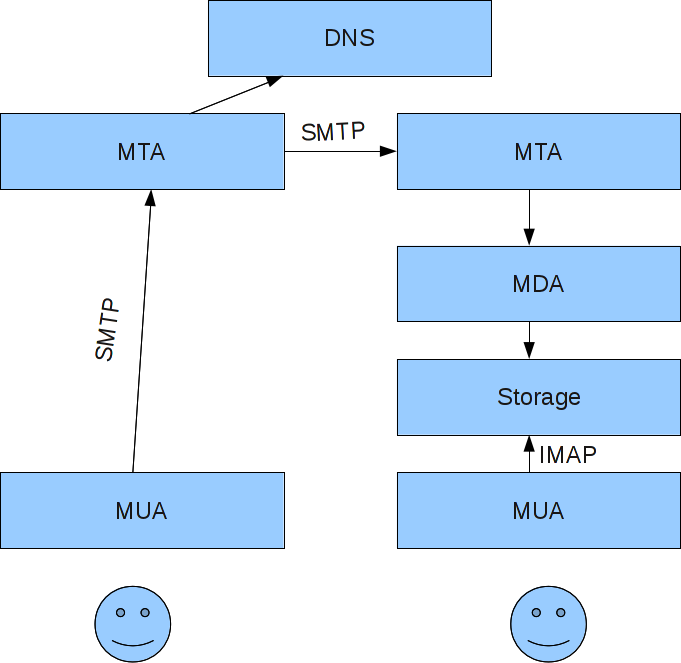
\includegraphics[width=10cm]{img/emailscheme}
\end{center}
\caption{Схема работы электронной почты. Меджду двумя агентами доставки почты (MTA) может находиться еще некоторое количество промежуточных серверов.}
\label{d_tree}
\end{figure}

\begin{enumerate}
\item почтовый клиент(Mail User Agent, MUA) пользователя $A$ инициирует соединение с сервером электронной почты (Mail Transporting Ageint, MTA) домена bar.net и передает ему письмо для b@example.com по протоколу SMTP.
\item Почтовый сервер домена bar.net запрашивает у своего DNS сервера информацию о домене example.com и выясняет адрес сервера, ответственного за обработку писем для домена example.com
\item Почтовый сервер домена bar.net инициирует соединение с почтовым сервером домена example.com и передает ему письмо по протоколу SMTP
\item Почтовый сервер домена example.com анализирует письмо, выясняет что домен адресата соответствует домену, который обслуживает этот сервер и иницирует соединение с агентом доставки почты (Mail Delivery Agent, MDA). Способ передачи письма от MTA к MDA не определен стандартом(например может использвоваться протокол доставки локальной почты LMTP - Local Mail Transfer Protocol).
\item MDA передает письмо в хранилище. Письмо хранится в хранилище до тех пор, пока почтовый клиент пользователя $B$ не инициирует соединение с ним и не заберет у него письмо. Для взаимодействия хранилища почты с почтовым клиентом обычно используются такие протоколы как IMAP4 или POP3
\end{enumerate}

\subsubsection{Где можно бороться со спамом}
Исходя из схемы работы электронной почты бороться со спамом можно в следующих местах:
\begin{itemize}
\item Компьютер отправителя. В последнее время большая часть спама рассылается с компьютеров, зараженным вредоносным программным обеспечением. Дл того чтобы этого не происходило на компьютере отправителя можно устанавливать различные антивирусы, блокировщики  траффика и другое ПО, помогающее защититься от вредоносных программ.
\item Шлюз провайдера. Провайдер отправителя может блокировать подключения, которые ,по его мнению, устанавливаются с целью рассылки спама.
\item Отправляющий SMTP-сервер. Может отказаться от передачи сообщения, если сочте, что письмо является спамом.
\item Принимающий SMTP сервер. Может отказаться от приема сообщения, может уведомить получателя о попытке передачи спама. Может лучше фильтровать сообщения с учетом особенностей конкретных пользователей.
\item Принимающий компьютер. Может проанализировать письмо и пометить его как спам. Необходима настройка фильтрации для каждой установки почтовой программы.

Фильтрация спама на потчовом сервере получателя представляет наибольший интерес, так как она имеет все достоинства фильтрации в почтовой программе получателя, и кроме того избавляет пользователя от необходимости \textbf{получать} нежелательные письма. В дальнейшем будем рассматривать именно фильтрацию на почтовом сервере получателя.
\end{itemize}

\subsection{Обзор методов машинного обучения} 
\subsubsection{Обучение по прецедентам}
Пусть есть неизвестная функция $F: X -> Y$, переводящая объекты
множества $X$ в объекты множества $Y$, причем для некторых $x_1, x_2, ... x_n$ известны соответсвующие им значения $y_1 = F(x_1), y_2 = F(x_2), ... y_n = F(x_n)$.
Необходимо построить функцию $F^*(X)$, наилучшим образом приближающую $F(X)$.

Под фразой \textbf{наилучшим образом приближает} подразумевается, что для некоторого функционала качества $\mu(y, y')$, матожидание
\begin{equation}
\label{}
E\mu(F(x), F^*(x)), x \in X
\end{equation}
будет минимальным.

В качестве $\mu(y, y')$ можно брать например модуль разности, квадрат разности и т. п.

\textbf{Методом обучения} называется проецесс построения $F^*(x)$ по известным парам $(x_1, y_1), (x_2, y_2), ... (x_n, y_n)$. Множество таких пар называется \textbf{обучающей разности}

Построенную функцию $F^*(x)$ часто также называют \textbf{алгоритмом}, подразумевая что она должна быть эффективно вычислима на компьютере.

Задача построения такого алгоритма не может быть решена точно, т. к. неизвестна природа исходной функции $F(x)$. Кроме того минимизация $\mu$ на обучающей выборке не обязательно приводит к тому, что и на новых обхектах из $X$ значение $\mu$ также будет мало.
%TODO смотри пример(рисунок, переобучение)

Процесс построения модели можно также рассматривать как выбор конкретного значения функции $F^*(x)$ из семейства $F^*(x, \pi)$. Значение выбранного параметра $\pi$ в таком случае называется \textbf{моделью} для алгоритма
$F^*(x)$

В целом процесс решения задачи машинного обучения называют \textbf{машинным обучением} или \textbf{обучением по прецедентам}

В зависимости от вида множества $Y$, задача может являться задачей классификации(множество конечно) или регрессии(множество бесконечно).
Задача фильтрации спама по своей сути является задачей классификации с двумя классами.

Объекты из множества $X$ обычно рассматривают как вектор в некотором $N$-мерном пространстве. Если изначально объекты имеют более сложную структуру(например текст, аудиозапись), то ее некоторым способом представляют в виде вектора. Элементы таких векторов называются \textbf{признаками}.

\subsubsection{Скользящий контроль}
Так как вид функции $F(X)$  неизвестен, то прямо посчитать значение матожидания \ref{matozh} не возможным. Для того чтобы хоть как-то оценить качество построенного алгоритма обычно пользуются методом \textbf{скользащего контроля}. Метод заключается в следующем: первоначальная обучающая выборка делится на несколько частей. Обучение проводится по очереди на каждой из частей, а значение $\mu$ оценивается по оставшимся частям.

Итоговую оценку $\mu$ считают как
\begin{equation}
\mu' = 1/n\sum_1^n{\mu_i}, i \in 1..n
\end{equation}

\subsubsection{Байесовские методы}
\subsubsection{Наивный байесовский классификатор}
\subsubsection{Нейронные сети}
Нейронная сеть — это математическая модель, а также ее программные или аппаратные реализации, построенная в некотором смысле по образу и подобию сетей нервных клеток живого организма.

Нейронные сети — один из наиболее известных и старых методов машинного обучения.

\subsubsection{Решающие деревья}
Решающие деревья представляют собой идейно достаточно простой метод обучения: строится дерево, в узлах которого ставятся некоторые предикаты(простые пороговые решающие правила). В листах этого дерева записываются значения $F^*(x)$, соответсвующие значеиниям предикатов.

Обычно такие деревья склонны к переобучению, однако существуют закрытые реализации алгоритмов классификации, в которых деревья используются в качестве базовых алгоритмов для более сложных алгоримов.
\begin{figure}[h]
\begin{center}
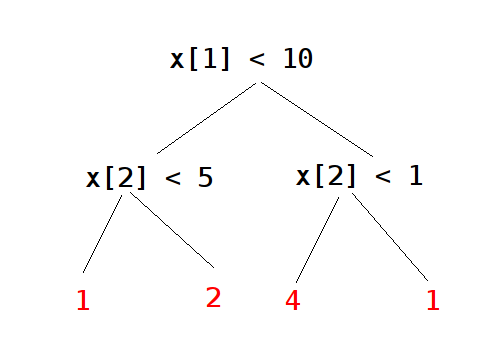
\includegraphics[width=10cm]{img/d_tree}
\end{center}
\caption{Решающее дерево: в узлах предикаты, в листьях значения целевой функции}
\label{d_tree}
\end{figure}

\subsubsection{Метод опорных векторов}
Метод опорных векторов основан на \textbf{принципе максимизации зазора}. Пусть стоит задача классификации с двумя классами. В пространстве признаков классифицируемых объектов проводится гиперплоскость таким образом, чтобы объекы обучающей выборки принадлежащие одному классу лежали по одну сторону от этой гиперплоскости, а объекты принадлежащие второму классу по другую.

Понятно, что если гиперплоскость существует, то она не единственна. Среди всех таких гиперплоскостей выбирается такая, которая максимизирует \textbf{зазор} -- минимальное расстояние от гиперплоскости до ближайшей точки обучающей выборки. Таким образом расстояние от гиперплоскости до ближайшего объекта каждого из классов будет одинаково.

\begin{figure}[h]
\begin{center}
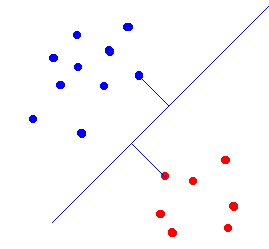
\includegraphics[width=5cm]{img/svm}
\end{center}
\caption{Наилучшая разделяющая прямая в двухмерном пространстве}
\label{svm}
\end{figure}

Если разделяющая гиперплоскость существует выборка называется \textbf{линейно разделимой}.

Для обобщения на случай линейно неразделимой выборки используется следующая идея: выборку можно сделать линейно разделимой, если увеличить размерность пространства. Для этого используется так называемая \textbf{ядерная функция}

\begin{figure}[h]
\begin{center}
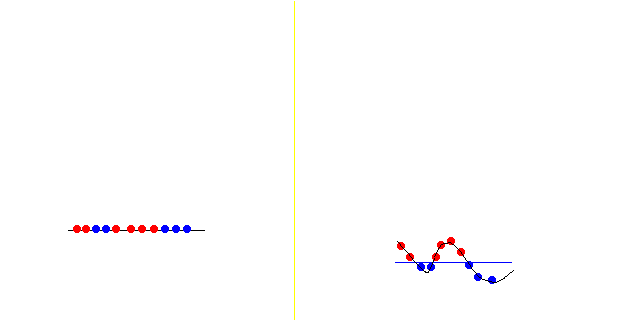
\includegraphics[width=15cm]{img/svm2}
\end{center}
\caption{Неразделимая в одномерном пространстве выборка стала разделимой после перевода в двумерное пространство}
\label{svm-kernel}
\end{figure}

Метод опорных векторов в настоящее время рассматривается как наиболее универсальный и хорошо работающий на большом количестве задач. Кроме того в работе А. Розинкина было показано что этот метод показывает хорошие результаты при применении его к задаче фильтрации спама. Для решения поставленной задачи мы также воспользуемся этим методом.

\subsection{Обзор существующих открытых систем фильтрации спама}
По требованию постановки задачи реализация должна быть выполнена в виде модификации одной из существующих систем фильтрации спама. В данном разделе будут приведены описания некоторых систем фильтрации спама и выбрано одно из них для дальнейшей модификации.
\subsubsection{spamassassin}
SpamAssassin - одно из наиболее известных открытых средств фильтрации спама. Этот проект динамично развивается и показывает хорошие результаты производительности и качества фильтрации. SpamAssassin использует в своей работе большое количество методик обнаружения спама.
\subsubsection{spambrobe}


\subsubsection{dspam}
\textbf{dspam} - открытая система фильтрации спама. Dspam изначально проектриовался для работы в многопользовательском режиме.
Для фильтрации спама dspam может использовать одну из нескольких разновидностей байесового классификатора.
Dspam написан на языке С и работает достаточно эффективно. Dspam имеет большое сообщество разработчиков и активно развивается в настоящий момент.
Из недостатков системы dspam можно отметить использование устаревшей системы сборки (autools) и использование низкоуровневой разработки, что усложняет понимание и модификацию его исходного кода.
Для доработки был выбран именно dspam, так как он удовлетворяет нашим требованиям, а именно:
\begin{itemize}
\item Ориентирован на работе на стороне сервера
\item Распространяется под свободной лицензией
\item Ориентирован на многопользовательский режим
\item Фильтрация спама осуществляется  всего одним алгоритмом, что упрощает тестирование разработанного метода
\end{itemize}
